% ============================================================
%  Příprava na maturitu – Elektrotechnika
%  Okruh 6: Transformátory
% ============================================================

\documentclass[a4paper,10pt]{article}

\usepackage[T1]{fontenc}
\usepackage[utf8]{inputenc}
\usepackage[left=2.0cm, right=1.8cm, top=1.8cm, bottom=1.8cm]{geometry}
\usepackage{parskip}
\usepackage{xcolor}
\usepackage{tabularx}
\usepackage{booktabs}
\usepackage{tikz}
\usepackage{mdframed}
\usepackage{amsmath}
\usepackage{enumitem}
\usepackage{circuitikz}

\usetikzlibrary{arrows.meta, positioning, decorations.pathmorphing, shapes.geometric, calc}

% --- Barvy ---
\definecolor{accent}{HTML}{1A3A5C}
\definecolor{lightblue}{HTML}{EAF2F8}
\definecolor{lightyellow}{HTML}{FDFBE4}
\definecolor{lightgreen}{HTML}{EAF7EA}
\definecolor{lightred}{HTML}{FDE8E8}
\definecolor{lightgray}{HTML}{F4F4F4}

% --- Boxy ---
\newmdenv[backgroundcolor=lightblue,linecolor=accent!40,roundcorner=4pt,
  innertopmargin=6pt,innerbottommargin=6pt,innerleftmargin=8pt,innerrightmargin=8pt]{pojmybox}
\newmdenv[backgroundcolor=lightyellow,linecolor=accent!30,roundcorner=4pt,
  innertopmargin=6pt,innerbottommargin=6pt,innerleftmargin=8pt,innerrightmargin=8pt]{vysvetlenibox}
\newmdenv[backgroundcolor=lightgreen,linecolor=accent!40,roundcorner=4pt,
  innertopmargin=6pt,innerbottommargin=6pt,innerleftmargin=8pt,innerrightmargin=8pt]{vzorcebox}
\newmdenv[backgroundcolor=lightred,linecolor=accent!30,roundcorner=4pt,
  innertopmargin=6pt,innerbottommargin=6pt,innerleftmargin=8pt,innerrightmargin=8pt]{durazbox}

\setlist[itemize]{noitemsep, leftmargin=1.4em, topsep=2pt}
\setlist[enumerate]{noitemsep, leftmargin=1.4em, topsep=2pt}

% --- Zkratka pro jednotky ---
\newcommand{\jednotka}[1]{\,[\mathrm{#1}]}

\begin{document}

% ============================================================
\section*{\large Okruh 6 – Transformátory}

\begin{pojmybox}
\textbf{Klíčové pojmy:}
transformátor, primární a sekundární vinutí, magnetický obvod, Faradayův zákon elektromagnetické indukce, převod transformátoru ($p$), ztráty v železe a v mědi, účinnost, galvanické oddělení, autotransformátor, měřicí transformátor
\end{pojmybox}

\begin{vysvetlenibox}

% ================================================================
\subsection*{1. Princip činnosti transformátoru}

Transformátor je netočivý elektrický stroj, který slouží k přeměně střídavého napětí a proudu na jiné hodnoty při zachování frekvence. 

\textbf{Princip:} Využívá Faradayův zákon elektromagnetické indukce (\textit{viz Okruh 3}).
\begin{enumerate}
  \item Střídavý proud $I_1$ v \textbf{primárním vinutí} vytvoří střídavý magnetický tok $\Phi$.
  \item Tento magnetický tok se uzavírá přes feromagnetické \textbf{jádro} (magnetický obvod).
  \item Proměnný tok $\Phi$ protíná \textbf{sekundární vinutí} a indukuje v něm střídavé napětí $U_2$.
\end{enumerate}

\begin{durazbox}
\textbf{Důležité:} Transformátor funguje \textbf{pouze na střídavý proud}! Připojením na stejnosměrné napětí (DC) by se indukovalo napětí jen při zapnutí/vypnutí, jinak by cívka působila jako zkrat a shořela by.
\end{durazbox}

\begin{center}
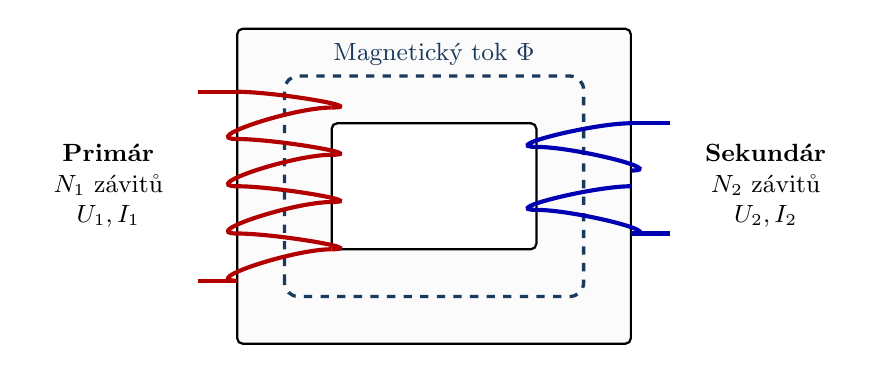
\begin{tikzpicture}[>=Stealth, font=\small, thick]
  % Jádro
  \draw[fill=lightgray!40, rounded corners=2pt] (0,0) rectangle (5,4);
  \draw[fill=white, rounded corners=2pt] (1.2,1.2) rectangle (3.8,2.8);
  
  % Magnetický tok (čárkovaně uvnitř)
  \draw[dashed, accent, line width=1.2pt, rounded corners=5pt, ->] 
    (0.6,0.6) rectangle (4.4,3.4);
  \node[accent, above] at (2.5,3.4) {Magnetický tok $\Phi$};

  % Primární vinutí (vlevo)
  \draw[red!70!black, line width=1.5pt] (-0.5, 3.2) -- (0, 3.2);
  \foreach \y in {3.2, 2.6, 2.0, 1.4} {
    \draw[red!70!black, line width=1.5pt] (0, \y) to[out=0, in=0] (1.2, \y-0.2);
    \draw[red!70!black, line width=1.5pt] (1.2, \y-0.2) to[out=180, in=180] (0, \y-0.6);
  }
  \draw[red!70!black, line width=1.5pt] (0, 0.8) -- (-0.5, 0.8);
  
  % Sekundární vinutí (vpravo)
  \draw[blue!70!black, line width=1.5pt] (5.5, 2.8) -- (5, 2.8);
  \foreach \y in {2.8, 2.0} {
    \draw[blue!70!black, line width=1.5pt] (5, \y) to[out=180, in=180] (3.8, \y-0.3);
    \draw[blue!70!black, line width=1.5pt] (3.8, \y-0.3) to[out=0, in=0] (5, \y-0.6);
  }
  \draw[blue!70!black, line width=1.5pt] (5, 1.4) -- (5.5, 1.4);

  % Popisky
  \node[left] at (-0.6, 2.0) {\begin{tabular}{c} \textbf{Primár}\\$N_1$ závitů\\$U_1, I_1$\end{tabular}};
  \node[right] at (5.6, 2.0) {\begin{tabular}{c} \textbf{Sekundár}\\$N_2$ závitů\\$U_2, I_2$\end{tabular}};
\end{tikzpicture}
\end{center}

Obě vinutí jsou od sebe \textbf{galvanicky oddělena} (nejsou vodivě spojena, výkon se přenáší pouze magnetickým polem). To má obrovský význam pro bezpečnost a ochranu proti rušení.

% ================================================================
\subsection*{2. Převod transformátoru}

Poměr mezi počtem závitů, napětím a proudem definuje tzv. \textbf{převod transformátoru} $p$. 
Ideální transformátor přenáší výkon beze ztrát ($P_1 = P_2 \implies U_1 \cdot I_1 = U_2 \cdot I_2$).

\begin{vzorcebox}
\[
p = \frac{U_1}{U_2} = \frac{N_1}{N_2} = \frac{I_2}{I_1}
\]
\end{vzorcebox}

\begin{itemize}
  \item \textbf{$p > 1$ (Transformace dolů):} $N_1 > N_2 \implies U_1 > U_2$. Napětí klesá, proud stoupá (např. svářečka, nabíječka).
  \item \textbf{$p < 1$ (Transformace nahoru):} $N_1 < N_2 \implies U_1 < U_2$. Napětí stoupá, proud klesá (např. v elektrárně pro přenos VVN).
  \item \textbf{$p = 1$ (Oddělovací transformátor):} $U_1 = U_2$. Slouží výhradně pro galvanické oddělení obvodů (např. v koupelnách pro holicí strojky).
\end{itemize}

% ================================================================
\subsection*{3. Ztráty v transformátoru a účinnost}

Žádný transformátor není ideální. Výkon na sekundáru je vždy menší o ztráty, které se mění v teplo. Ztráty dělíme do dvou hlavních skupin:

\begin{enumerate}
  \item \textbf{Ztráty v železe ($\Delta P_{Fe}$ / Ztráty naprázdno):} Vznikají v magnetickém jádře vlivem vířivých proudů a hystereze (\textit{přemagnetování, viz Okruh 3}). Omezují se stavbou jádra ze vzájemně izolovaných transformátorových plechů. Nezávisí na zatížení, jsou konstantní.
  \item \textbf{Ztráty v mědi ($\Delta P_{Cu}$ / Ztráty nakrátko):} Vznikají jako Jouleovo teplo na ohmickém odporu primárního a sekundárního vinutí ($R \cdot I^2$). Rostou se čtvercem odebíraného proudu (čím více zátěže, tím víc hřeje).
\end{enumerate}

\begin{vzorcebox}
\[
\text{Účinnost:} \quad \eta = \frac{P_{out}}{P_{in}} = \frac{P_2}{P_1} = \frac{P_2}{P_2 + \Delta P_{Fe} + \Delta P_{Cu}} \cdot 100 \jednotka{\%}
\]
\end{vzorcebox}
\textit{Poznámka: Velké energetické transformátory mají účinnost vynikající, často přes 98 \%.}

% ================================================================
\subsection*{4. Trojfázové transformátory}

Používají se v energetice. Mají magnetický obvod se třemi sloupky. Na každém sloupku je navinut primár i sekundár jedné fáze. 
Vinutí lze zapojit do \textbf{hvězdy (Y)} nebo \textbf{trojúhelníku (D)} – \textit{bude úzce souviset s Okruhem 9 (Rozvodná soustava)}.
Značí se například Yy0 nebo Dyn1 (velké písmeno pro primár, malé pro sekundár, číslo udává fázový posun v hodinách - tzv. hodinový úhel).

% ================================================================
\subsection*{5. Speciální transformátory}

\subsubsection*{Autotransformátor}

Na rozdíl od klasického transformátoru má autotransformátor \textbf{pouze jedno společné vinutí}. Primár a sekundár nejsou galvanicky odděleny.

\begin{center}
\begin{circuitikz}[font=\small, thick]
  \draw (0,0) to[short, o-] (2,0) to[L, l=$N_1$, *-*] (2,4) to[short, -o] (0,4);
  \node[left] at (0,2) {$U_1$};
  
  % Odbočka sekundáru
  \draw (2,1.5) to[short, *-o] (4,1.5);
  \draw (2,0) to[short, -o] (4,0);
  
  \node[right] at (4,0.75) {$U_2$};
  \node[right] at (2.2, 0.75) {$N_2$};
  
  \draw[<->, dashed, accent] (0, 0.2) -- (0, 3.8);
  \draw[<->, dashed, accent] (4, 0.2) -- (4, 1.3);
\end{circuitikz}
\end{center}

\textbf{Výhody:} Úspora mědi (menší rozměry a hmotnost při stejném výkonu), nižší ztráty. Často se používá jako regulační (laboratorní autotransformátor / variak) s pohyblivým jezdcem.
\textbf{Nevýhody:} Chybí galvanické oddělení! Při přerušení společné části se na sekundáru objeví plné primární napětí (nebezpečí úrazu).

\subsubsection*{Měřicí transformátory (MTP a MTN)}
Slouží k měření velkých proudů a napětí pomocí běžných měřicích přístrojů.
\begin{itemize}
  \item \textbf{Měřicí transformátor napětí (MTN):} Převádí VVN na standardizovaných 100\,V. Sekundár nesmí být nikdy spojen nakrátko.
  \item \textbf{Měřicí transformátor proudu (MTP):} Převádí obrovské proudy (např. 1000\,A) na standardizovaných 5\,A nebo 1\,A. Primár tvoří často jen jeden průvlak silového kabelu toroidem. \textbf{Pozor:} Sekundár MTP nesmí být nikdy rozpojen (naprázdno), jinak na něm vznikne nebezpečné přepětí, které ho zničí!
\end{itemize}

% ================================================================
\subsection*{6. Shrnutí – přehled vzorců}

\begin{center}
\begin{tabularx}{0.97\linewidth}{@{} l l l @{}}
\toprule
\textbf{Veličina} & \textbf{Vzorec} & \textbf{Jednotka} \\
\midrule
Převod transformátoru & $p = \dfrac{U_1}{U_2} = \dfrac{N_1}{N_2} = \dfrac{I_2}{I_1}$ & -- \\
Účinnost & $\eta = \dfrac{P_2}{P_1} = \dfrac{P_2}{P_2 + \Delta P_{Fe} + \Delta P_{Cu}}$ & -- (nebo \%) \\
Činný výkon & $P = U \cdot I \cdot \cos \varphi$ & W (watt) \\
Zdánlivý výkon & $S = U \cdot I$ & VA (voltampér) \\
\bottomrule
\end{tabularx}
\end{center}

\end{vysvetlenibox}

\end{document}